% !TEX root = owasp-doc.tex

% ================================================
%	LLM Challenges
% ================================================

\headerimage

\chapter{Large Language Model Challenges}

Large Language models face a number of serious and unique issues. One of the
most important is that while working with LLMs, the control and data planes
cannot be strictly isolated or separable. Another significant challenge is
that LLMs are nondeterministic by design, yielding a different outcome when
prompted or requested. It is not always a challenge, but LLMs employ semantic
search rather than keyword search. The key distinction between the two is that
the model's algorithm prioritizes the terms in its response. This is a
significant departure from how consumers have traditionally used technology,
and it has an impact on the consistency and reliability of the findings.
Hallucinations, emerging from the gaps and training flaws in the data the model
is trained on, are the result of this method.

There are methods to improve reliability and reduce the attack surface for
jailbreaking, model tricking, and hallucinations, but there is a trade-off
between restrictions and utility in both cost and functionality.

LLM use and applications increase an organization's attack surface. Some risks
associated with LLMs are unique, but many are familiar issues, such as the
known software bill of materials (SBOM), supply chain, data loss protection
(DLP), and authorized access. There are also increased risks not directly
related to GenAI, but GenAI increases the efficiency, capability, and
effectiveness of attacks.

Adversaries are increasingly harnessing LLM and Generative AI tools to refine
and expedite traditional methods. These enhanced techniques allow them to
effortlessly craft new malware, potentially embedded with novel zero-day
vulnerabilities or designed to evade detection. They can also generate
sophisticated, unique, or tailored phishing schemes. The creation of convincing
deep fakes, whether video or audio, further facilitates their social
engineering ploys. Additionally, these tools enable them to execute intrusions
and develop innovative hacking utilities. It is very likely that in the future,
more “tailored” and compound use of AI technology by criminal actors will demand
specific responses and dedicated solutions for appropriate defense schemas.

\clearpage

\section{LLM Threat Categories}

\begin{figure}[h]
  \centering
  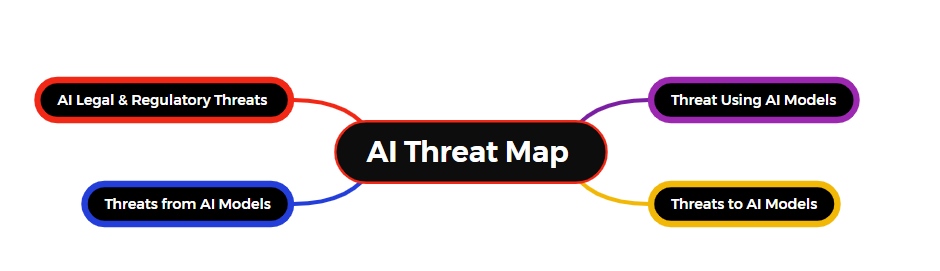
\includegraphics[width=\textwidth]{ai_threat_map}
  \caption{Image of types of AI threats}
  \label{fig:ai-threat-map}
\end{figure}

\section{Artificial Intelligence Security and Privacy Training}

Employees throughout organizations benefit from training to understand
artificial intelligence, generative artificial intelligence, and the future
potential consequences of building, buying, or utilizing LLMs. Training for
permissible use and security awareness should target all employees as well as
be more specialized for certain positions such as human resources, legal,
developers, data teams, and security teams.

Fair use policies and healthy interaction are key aspects that, if incorporated
from the very start, will be a cornerstone to the success of future AI
cybersecurity awareness campaigns. This will necessarily imply the user's
knowledge of the basic rules for interaction as well as the ability to separate
good behavior from bad or unethical behavior.

\section{Incorporate LLM Security and governance with Existing, Established Practices and Controls}

While AI and generated AI add a new dimension to cybersecurity, resilience,
privacy, and meeting legal and regulatory requirements, the best practices that
have been around for a long time are still the best way to find risks, test
them, fix them, and lower them.

\begin{itemize}
  \item The management of artificial intelligence systems is integrated with
  existing organizational practices.
  \item Apply existing privacy, governance, and security practices.
\end{itemize}

\clearpage

\section{Fundamental Security Principles}

LLM capabilities introduce a different type of attack and attack surface. LLMs
are vulnerable to complex business logic bugs, such as prompt injection,
insecure plugin design, and remote code execution. Existing best practices are
the best way to solve these issues. An internal product security team that
understands secure software review, architecture, data governance, and
third-party assessments The cybersecurity team should also check how strong
the current controls are to find problems that could be made worse by LLM,
like voice cloning, impersonation, or getting around captchas.

Accounting for the specific skills and competences developed in the last few
years around machine learning, NLP and NLU, deep Learning and lately, LLMs and
GenAI, it is advised to have skilled professionals with practice, knowledge, or
experience in these fields to side with security teams in adopting, at best,
and even shaping new potential analyses and responses to those issues.

\section{Risk}

Reference to risk uses the ISO 31000 definition: Risk = "effect of uncertainty on objectives."
LLM risks included in the checklist include a targeted list of LLM risks that
address adversarial, safety, legal, regulatory, reputation, financial, and competitive risks.

\section{Vulnerability and Mitigation Taxonomy}

Established methods of vulnerability classification and threat sharing are in
early development, such as Oval, STIX, threat sharing, and vulnerability
classification. The checklist anticipates calibrating with existing,
established, and accepted standards, such as CVE classification.
